\documentclass{apa}

% ---------- watermark -----------
\usepackage[firstpage]{draftwatermark}
\SetWatermarkAngle{0}
\SetWatermarkFontSize{0.25cm}
\SetWatermarkVerCenter{1.15cm}
\SetWatermarkLightness{0.5}
\SetWatermarkHorCenter{14cm}
\SetWatermarkText{\shortstack[l]{
Perfors, A. and Navarro, D. J. (2014). Language evolution can be shaped
by the structure of the world. Cognitive Science, 38, 775-793.\\
http://dx.doi.org/10.1111/cogs.12102
}}
\SetWatermarkScale{1}
% -------------------------------

%\usepackage[dvips]{epsfig}
\usepackage{graphicx}
\usepackage{lscape}

	\usepackage{bm}
	\usepackage{apacite}

%\newcommand{\p}{P}
%\newcommand{\xn}{{\bm{x}}}
%\newcommand{\rt}{{r_t}}
%\newcommand{\htr}{{h_t}}
%\newcommand{\condon}{\, | \,}
%\newcommand{\pgap}{\,}

\title{Language evolution can be shaped by the structure of the world}

\twoauthors{\normalsize Amy Perfors}{\normalsize Danielle J. Navarro}
\twoaffiliations{School of Psychology \\ University of Adelaide \\ +618 8313 5744 \\ amy.perfors@adelaide.edu.au}{School of Psychology \\ University of Adelaide}

\raggedbottom
\interfootnotelinepenalty=10000

\abstract{Human languages vary in many ways, but also show striking cross-linguistic universals. Why do these universals exist? Recent theoretical results demonstrate that Bayesian learners transmitting language to each other through iterated learning will converge on a distribution of languages that depends only on their prior biases about language and the quantity of data transmitted at each point; the structure of the world being communicated about plays no role (Griffiths \& Kalish, 2005, 2007). We revisit these findings and show that when certain assumptions about the the relationship between language and the world are abandoned, learners will converge to languages that depend on the structure of the world as well as their prior biases. These theoretical results are supported with a series of experiments showing that when human learners acquire language through iterated learning, the ultimate structure of those languages is shaped by the structure of the meanings to be communicated.\\
{\bf Keywords:} language evolution; iterated learning; linguistic structure}

\begin{document}
\maketitle

\section{Introduction}

Human languages have rich structure on many levels, from phonology to semantics to grammar. Where does this structure come from? Many researchers agree that linguistic structure is shaped by the structure of our minds -- that our brains contain prior biases that favor the acquisition or retention of some linguistic systems over others. As such, debate generally centers around the nature and origin of these biases. Some suggest that natural selection operates on genes for language \cite{pinkerbloom90,nowaketal01,komarovanowak01} or on capabilities then used by the language faculty \cite{hauseretal02}. Others have suggested that humans easily learn language not because of a language-specific genetically encoded mechanism, but because language evolved to be learnable and usable by human brains \cite{zuidema02,brightonetal05b,christiansenchater08}. While these accounts disagree in many particulars, they agree that the structure of language arises from the structure of the brain.

In this paper we argue that language evolution can be shaped by the structure of the world in addition to pre-existing cognitive biases. Because language involves communicating about the world, the structure of that world (i.e., the things to be communicated) can interact with people's prior biases to shape the languages that develop. We offer theoretical and experimental support of this proposition. On the theoretical side, we take as our starting point recent work within the ``iterated learning'' framework (in which new learners receive their data from previous learners). Previous research has shown that when learners are individually Bayesian, an iterated learning chain converges in the limit to the prior distribution over all possible languages \cite{griffithskalish05,griffithskalish07}.  However, the proof of this rests on certain premises: either languages carry no assumptions about the distribution of meanings/events in the world \cite{griffithskalish05}, or if they do, the frequency with which those events are spoken about is entirely dependent on the language, rather than also the distribution of events in the world \cite{griffithskalish07}. Here we demonstrate that if either premise is abandoned, the iterated learning process converges to a distribution that depends on the distribution of events in the world as well as the prior biases of the learner. These theoretical results are experimentally tested in a lab-based iterated learning experiment, as in \citeA{kirbyetal08}, which shows that participants converge on different languages depending on the structure of the space of meanings they are shown.


\subsection{Iterated learning}

\begin{figure}[t]
\begin{center}
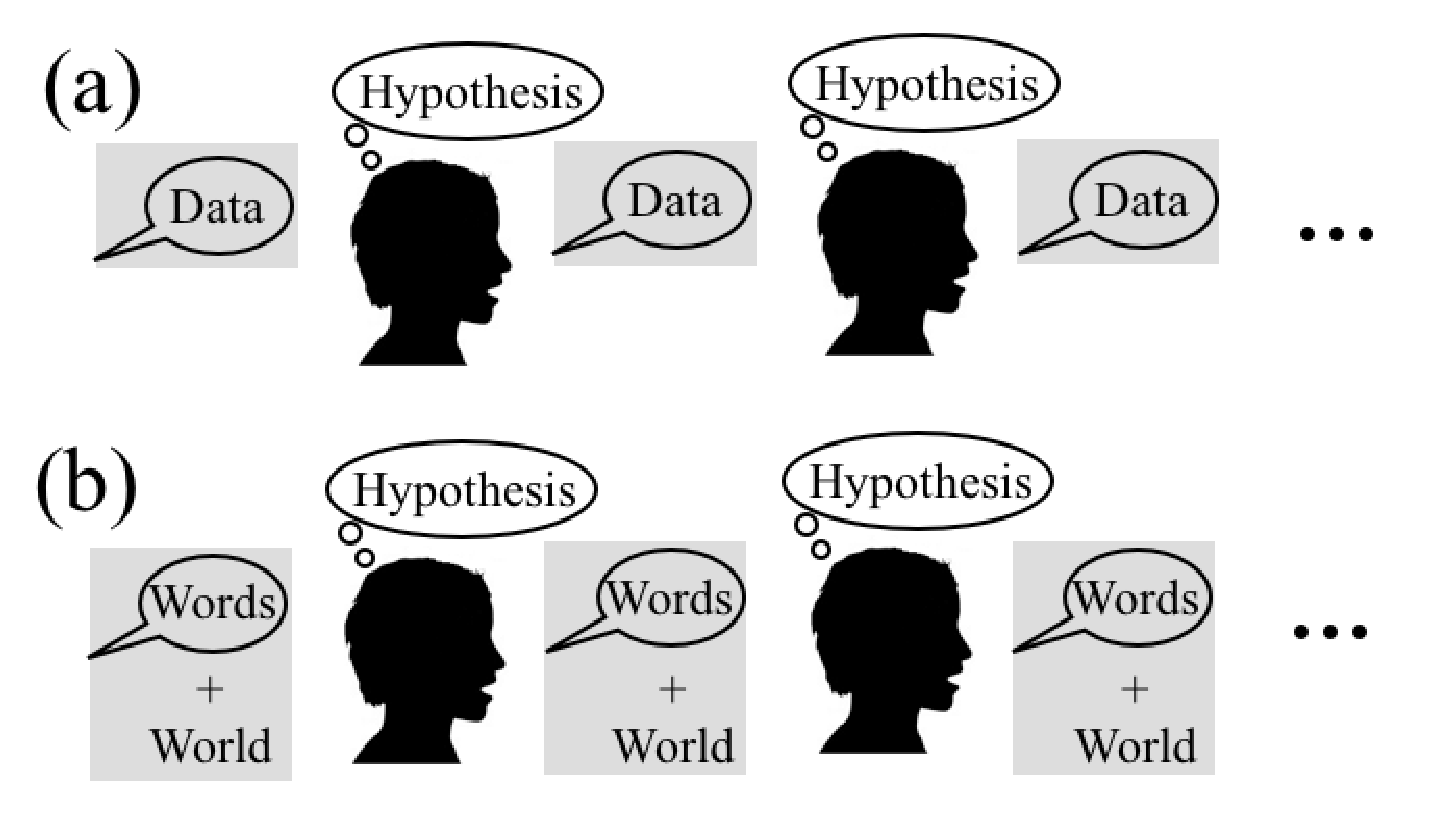
\includegraphics[scale=0.5]{ilframework.eps}
\end{center}
\vspace{-5mm}
\caption{(a) Schematic illustration of the typical iterated learning paradigm, which assumes that learner $n$ acquires language on the basis of the language data produced by learner $n-1$. (b) A different view of iterated learning recognizes that because individuals produce language in order to communicate about the world, the data available to learners includes meanings in the world as well as the linguistic data produced by the learner before them.}
\label{fig:ilm}
\end{figure}


The iterated learning modeling (ILM) framework is widely used in language evolution research \cite{griffithskalish07, kirbyetal08,kirbyhurford02,smith09,realigriffiths09}. It views the process of language evolution in terms of a chain of Bayesian learners (or generations), which is illustrated schematically in Fig.~\ref{fig:ilm}. The first learner in the chain sees some linguistic data (e.g., utterances), forms a hypothesis about what sort of language would have generated that data, and then produces their own data by sampling from their posterior distribution; this data then serves as input to the next learner in the chain. Over time, the languages that emerge from this process become non-arbitrary: two recent papers (both referred to, henceforth, as GK) demonstrate that when the learners are Bayesian, we should expect an iterated learning chain to converge to the prior distribution over all possible languages \cite{griffithskalish05,griffithskalish07}. That is, the probability of any given language emerging does not depend on the structure of the world or independent properties of the language -- only the assumptions of the learner. The existence of a linguistic bottleneck (in which only a small amount of information is transmitted at each link in the chain) can speed the rate of convergence, but GK's result implies that neither the structure of the meaning space nor the nature of the initial language should have an effect on the language that eventually evolves.

\vspace{5mm}
------------------------------ Insert Figure~\ref{fig:ilm} about here -------------------------------
\vspace{5mm}

\begin{figure}
\begin{center}
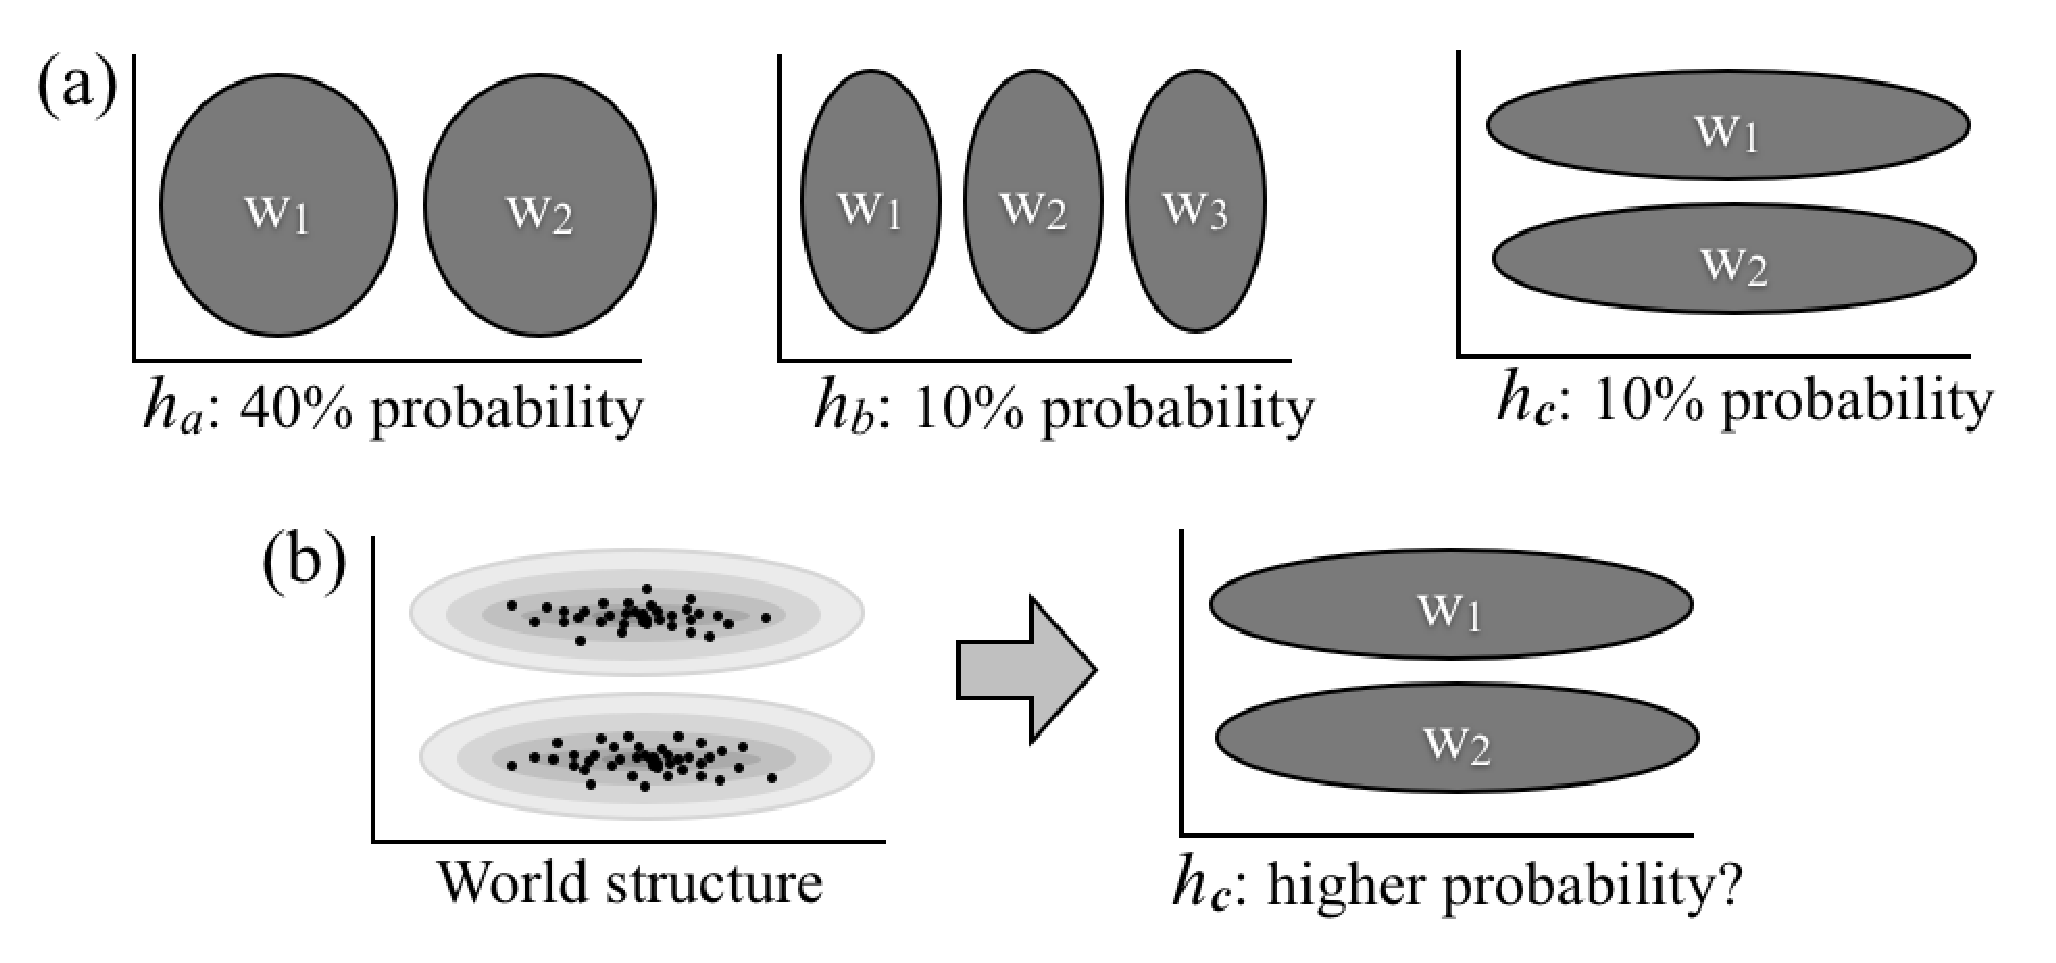
\includegraphics[scale=0.45]{circles.eps}
\end{center}
\vspace{-5mm}
\caption{(a) Intuitive illustration of the results of Griffiths \& Kalish 2005, 2007 (GK). Given a 2-dimensional semantic space, a learner with a prior bias to favor one dimension of that space (the $x$-axis) and languages with fewer words might have a prior distribution over languages that puts more probability on $h_a$ and less on $h_b$ or $h_c$. GK demonstrate that the languages that evolve will converge to this prior distribution. (b) However, if the natural categories in the world have a different structure, we might intuitively expect that languages that capture that structure, like $h_c$, should be more likely to evolve.}
\label{fig:circles}
\end{figure}


GK's result can be conceptualized as follows. Suppose learners must acquire languages that describe a two dimensional semantic space of some sort. For illustrative purposes, suppose further that the learners have a prior bias to prefer languages with fewer words and to pay more attention to one of the dimensions, as occurs in human category learning and development \cite{landauetal88}.  This prior bias might impose a distribution over hypotheses $h$ about possible languages, like the illustrative one shown in Fig.~\ref{fig:circles}(a): languages like $h_a$ with a few words that classify according to the preferred dimension (the $x$-axis in this case) have higher prior probability than languages like $h_b$, which have many words, or $h_c$, whose words classify according to the dis-preferred dimension. GK suggest that languages evolving to describe this space will converge to the prior distribution: 40\% of the time $h_a$ will emerge, 10\% of the time $h_b$ will emerge, and so forth. Although this prior and these precise numbers are imaginary, the picture shown in Fig.~\ref{fig:circles}(a) provides a schematic illustration of what GK's results mean.

\vspace{5mm}
------------------------------ Insert Figure~\ref{fig:circles} about here -------------------------------
\vspace{5mm}

It also, however, highlights an apparent oddity within these results. Suppose that the world possesses structure in the form of natural categories of some sort, and these natural categories happen to group items according to the non-preferred dimension, as shown in Fig.~\ref{fig:circles}(b): the items observed by the learner -- generated by the world -- correspond to the black dots, which fall naturally into two clusters. We might intuitively expect that a language like $h_c$ would be a better fit to this world (and hence be more likely to evolve) than a language like $h_a$, even though $h_a$ has higher prior probability. The results of GK appear to suggest otherwise. Is our intuition simply wrong, or is there a mismatch between the GK derivation and the problem of language evolution within a structured world? In the next section, we argue for the latter.

\section{Theoretical result}

Our primary result formalizes the learning framework similarly to \citeA{griffithskalish05}, although later we will also address the slightly different formalization of \citeA{griffithskalish07}. For now, we consider a Bayesian learner who sees $m$ meanings or events, denoted $x = \{x^{(1)}\ldots x^{(m)}\}$. These meanings are paired with $m$ corresponding utterances denoted $y = \{y^{(1)}\ldots y^{(m)}\}$.  The first learner in the chain is shown some initial data consisting of meaning-utterance pairs $(x_0,y_0)$.
Then, when shown new events $x_1$, the learner produces utterances $y_1$, so that $(x_1,y_1)$ are the input to the next learner. In general, learner $n+1$ sees data $(x_n,y_n)$ and generates $y_{n+1}$ given events $x_{n+1}$, so that the next learner receives input $(x_{n+1},y_{n+1})$. The goal of each learner is to estimate the mapping between meanings and utterances, which corresponds to learning the language they are exposed to.
It is assumed that each learner has the same countable hypothesis space $\mathcal{H}$ of possible languages, such that each $h \in \mathcal{H}$ corresponds to one language. For any learner, acquisition involves a learning step and a production step.

In the {\bf learning step}, learner $n+1$ sees $(x_n,y_n)$ and computes a posterior distribution over possible languages $h_{n+1}$. Bayes' rule implies that we can express this posterior distribution as follows:

\begin{equation}
P(h_{n+1}|x_n,y_n) = \frac{P(y_n|x_n,h_{n+1}) P(h_{n+1}|x_n)}{\sum_{h \in \mathcal{H}} P(y_n|x_n,h) P(h|x_n)}
\label{eq:ourlearning1}
\end{equation}

\noindent
In their derivation, \citeA{griffithskalish05} assume that each language $h$ makes no assumption about which events $x$ are more likely than any other; given that assumption, they note that
$P(h|x) = P(h)$, and proceed with a version of Equation~\ref{eq:ourlearning1} based on that modification. Alternatively, however, it might be that the language carries with it certain assumptions about what events are possible or probable in the world, in which case the GK assumption is untenable.\footnote{More formally, GK assume that each language $h$ specifies $P(y | h,x)$, the {\it conditional} distribution over utterances $y$ given the events $x$. Our formulation corresponds to assuming that each language maps onto a {\it joint} (subjective) probability distribution over events and utterances, $P(x,y | h)$. We can factorize the joint distribution $P(x,y | h) = P(y | x,h) P(x | h)$. Moreover, since $P(h | x) \propto P(x | h) P(h)$, in our set up $P(h|x) \neq P(h)$.} In other words, simply observing meaningful events $x$ may bias the learner to prefer some languages over others.  If this is the case, then $P(h|x)$ does not equal $P(h)$, and the learning step is described by Equation~\ref{eq:ourlearning1}.

To see what this shift does to the iterated learning chain, we now turn to the {\bf production step}. In this step, the learner encounters new meanings $x_{n+1}$, generated from the (objective) distribution $Q(x)$ of meanings in the world. Given these meanings, the learner generates the new utterances $y_{n+1}$ by sampling them from $P(y_{n+1}|x_{n+1},h_{n+1})$, where $h_{n+1}$ is the learner's language (assumed to be sampled from the posterior distribution in Equation~\ref{eq:ourlearning1}).

Since all people in the chain follow the same learning and production steps, we can calculate $P(h_{n+1} | h_n)$, the probability that learner $n+1$ acquires language $h_{n+1}$ given that the previous learner used the language $h_n$, in the following way:
%%
\begin{equation}
P(h_{n+1}|h_n) = \displaystyle\sum_{x \in \mathcal{X}} \displaystyle\sum_{y \in \mathcal{Y}} P(h_{n+1}|x,y) P(y|x,h_n) Q(x).
\label{eq:trans}
\end{equation}
%%
Thus we have a sequence of random variables $h_1, h_2, h_3, \ldots$ describing the languages acquired by each person in the chain. This is constitutes a Markov chain whose transition probabilities are given by $P(h_{n+1}|h_n)$. Assuming the chain is ergodic, then its stationary distribution $\pi(h)$ satisfies
%%
\begin{equation}
\pi(h_{n+1}) = \displaystyle \sum_{h_n \in \mathcal{H}} P(h_{n+1}|h_n) \pi(h_n)
\label{eq:trans2}
\end{equation}
%%
\noindent
for all $h_{n+1}$. Put another way, the probability distribution over languages $h_n$ approaches $\pi(h_n)$ as $n \rightarrow \infty$.

In the setup used by \citeA{griffithskalish05}, the stationary distribution $\pi(h)$ corresponds to the prior $P(h)$. However, under our formalization this is no longer the case. To find the stationary distribution in this situation, we make the following ``representativeness'' assumption: that the posterior probability of a hypothesis given an actual dataset $x$ is close to its expected posterior probability given the generating distribution $Q(x)$. In other words, we assume that $P(h|x) \approx E_{Q(x^\prime)}[P(h | x^\prime)] = \sum_{x^\prime} P(h | x^\prime) Q(x^\prime)$, for some $x \sim Q(x)$.  If this assumption holds, then the stationary distribution is approximately $\pi(h) = \sum_x P(h | x) Q(x)$. That is, the chain converges to the {\it expected posterior distribution} over languages given meaningful events in the world. This is because for $\pi(h) = \sum_x P(h | x) Q(x)$ to be the stationary distribution it must be true that:

\footnotesize
\begin{eqnarray*}
\pi(h_{n+1})
&=& \sum_{h_n} P(h_{n+1} | h_n) \pi(h_n) \\
&=& \sum_x \sum_y \sum_{h_n} P(h_{n+1} | x, y) P(y | x, h_n) Q(x) \pi(h_n) \\
&=& \sum_x \sum_y \sum_{h_n} P(h_{n+1} | x, y) P(y | x, h_n) Q(x) \sum_{x^\prime} P(h_n | x^\prime) Q(x^\prime) \\
&\approx& \sum_x \sum_y \sum_{h_n} P(h_{n+1} | x, y) P(y | x, h_n) Q(x) P(h_n | x) \\
&=& \sum_x \sum_y  P(h_{n+1} | x, y)  Q(x) \sum_{h_n}  P(y | x, h_n) P(h_n | x) \\
&=& \sum_x \sum_y  P(h_{n+1} | x, y)  Q(x) P(y |x) \\
&=& \sum_x Q(x) \sum_y  P(h_{n+1} | x, y)  P(y |x) \\
&=& \sum_x Q(x)  P(h_{n+1} | x) \\
&=& \pi(h_{n+1})
\end{eqnarray*}
\normalsize

The assumption these results depend on is relatively weak: all it requires is that the events or meanings each learner sees be a representative sample from the true generating distribution $Q(x)$.\footnote{Note that this is actually a specific case of a more general result: languages may be shaped by world structure even in situations where the meanings are not a representative sample from $Q(x)$. We focus on the special case when representativeness holds because it does hold in a lot of situations and the stationary distribution is more interpretable in this case. Appendix A presents the more general proof.} In the limit where no learner sees any data, the stationary distribution converges to the prior, since $P(h | x) = P(h)$ in that situation. But as the amount of data increases, the languages that evolve will depend on the posterior distribution $P(h|x)$ and the distribution of meanings in the world $Q(x)$. Since the posterior depends on both prior and likelihood ($P(h|x) \propto P(h)P(x|h)$), this means that the languages that evolve will be sampled from a distribution depending on which ones are favored {\em a priori} as well as which ones best capture the meanings in the world. The additional $Q(x)$ term means that the distribution of those meanings matters as well. These results suggest that languages like $h_c$ might be more likely to evolve in a world like the one in Fig.~\ref{fig:circles}(b) than the prior distribution over languages might suggest.

The derivation offered by \citeA{griffithskalish07} removes the premise made by \citeA{griffithskalish05} that languages $h$ and events $x$ are independent. However, their new proof of convergence to the prior depends on a different premise: that when $h$ and $x$ are not independent, then the distribution of events $x$ depends entirely upon the language rather than the world.\footnote{More formally, this derivation assumes that data $d$ are generated from $P(d|h)$ and that $h$ are sampled from $P(h|d)$, for {\em any} construal of $d$. Thus, $d$ can include events $x$ as well as utterances $y$. Note that if $d = (x,y)$, however, the events and utterances are entirely generated by $P(d|h) = P(x,y|h)$: that is, an external event-generating distribution like $Q(x)$ plays no role.} Indeed, the 2007 derivation makes no reference to an external generating distribution, like $Q(x)$, at all.

Our results taken together with both GK derivations lead to the following conclusion: language evolution should by affected by the structure of the world as long as: (a) different languages make different predictions about the distribution of events, and (b) the actual distribution of which events are spoken about {\it does} depend, at least in part, on the nature of the external world. This second premise, put another way, simply states that language is shaped by the structure of the world as long as which things people talk about (and how often they talk about them) is affected by the distribution of those things in the external world, not just the language the people speak.

One key difference between our result and both GK results is that we predict that the amount of data that is transmitted from one speaker to the next (i.e., the information bottleneck) actually changes the stationary distribution of the chain. This contrasts with the prediction made by the GK derivations that while smaller bottlenecks lead to faster convergence, the language will always be a sample from the prior distribution over languages regardless of bottleneck size.\footnote{The GK results {\it do} predict that there will be an effect of bottleneck size if one assumes that learners are selecting the hypothesis with the maximum posterior probability (MAP estimation) rather than sampling directly from the posterior distribution \cite{griffithskalish07}. However, that bottleneck effect is different than the one we predict; it suggests, unlike us, that the stationary distribution will still always be centered on the prior, implying that the bottleneck size does not influence which language is most likely. The difference is that under MAP estimation, the variance of that distribution depends on the bottleneck size.} Our results, however, predict that the nature of the emergent languages will change as a function of the size of the bottleneck. When it is large or non-existent (i.e., there is a great deal of data available to each learner), the stationary distribution will converge to the expected posterior distribution over languages given meaningful events in the world; when the bottleneck is small, it will converge to the prior. This provides a natural test of our prediction: when the bottleneck is small, do the resulting languages resemble the ones that emerge when it is not?

In the next section we report experimental results supporting our theoretical findings. When there is a great deal of data available to the learner at each generation, the languages that emerge from an iterated learning chain with humans are shaped by the structure of the world. However, when there is little data, they look substantially different, and appear unaffected by the structure of the world. This is consistent with the predictions of our theoretical analysis but not that of GK.

\section{Method}

We adopt the standard iterated learning paradigm, in which participants form chains in which the output of the $n$th participant is the input of participant $n+1$ and the input for the first participant is random.  In a training phase, participants see a number of meaning-word pairs and are asked to learn them. In a test phase, they are shown meanings and asked to produce the corresponding word; these are the pairings for the next participant and correspond to the ``language'' that exists at that point in the chain. Our question is whether the languages that evolve over the course of a chain depend on the distribution of meanings $Q(x)$, and whether the predicted dependence on bottleneck size is observed.

 \subsection{Participants}

225 participants from the University of Adelaide participated in what they were told was an ``alien language'' study in which they were asked to learn a language consisting of labels for visual stimuli (squares of different sizes). Participants consisted of undergraduates from all departments as well as some recruited from a paid participant pool drawing from the surrounding community. The experiment was conducted at a computer terminal and the instructions did not reveal that it was an iterated learning experiment; participants did not know that their answers were to be given to the next participant.

\subsection{Stimuli}

The ``meanings'' in our experiments consisted of 36 possible squares differing in size and color, as shown in Fig.~\ref{fig:exptstimuli}(a). In the {\sc control} condition, color varied continuously from 0\% brightness (black) to 100\% brightness (white) in increments of 20\%, and size from smallest (10x10) to largest (60x60) in increments of 10 pixels.  In this condition there is no obvious or privileged way of categorizing the stimuli. In the {\sc size} condition, the stimuli were more discontinuous along the size dimension: the sizes were 10x10, 15x15, 20x20, 50x50, 55x55, and 60x0. In the  {\sc color} condition they were discontinuous along the color dimension: the colors were 0\%, 10\%, 20\%, 80\%, 90\%, and 100\% brightness.

\begin{figure}
\begin{center}
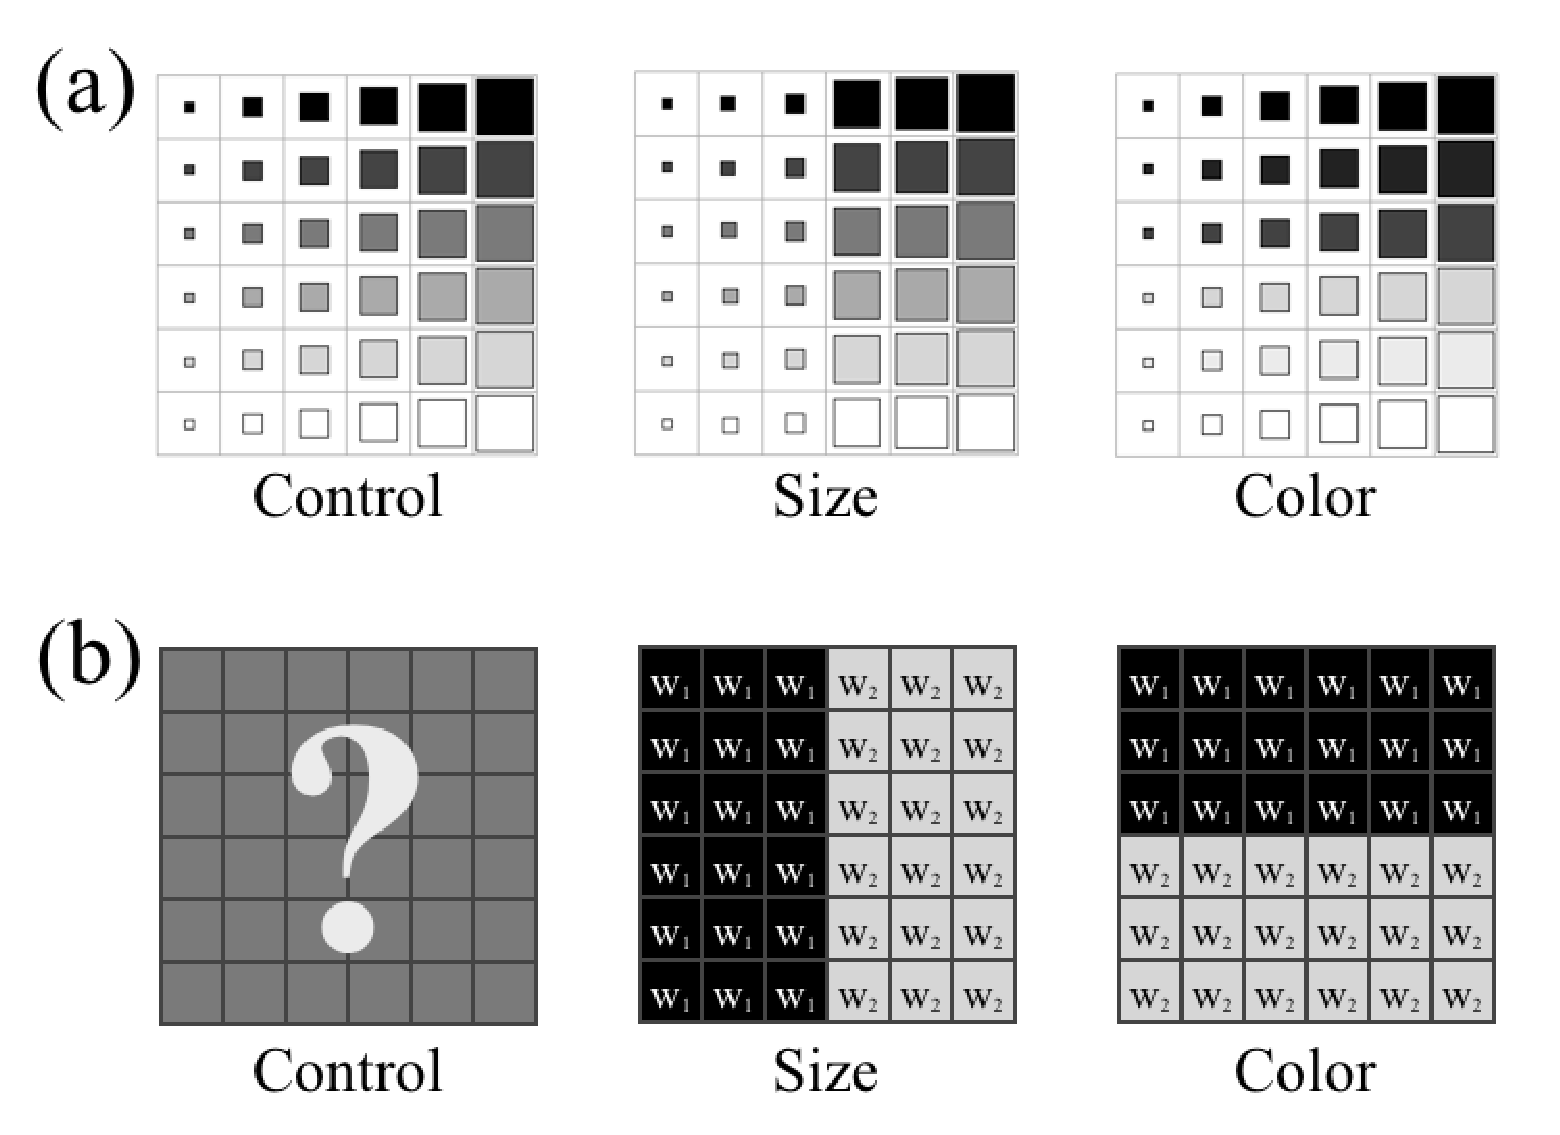
\includegraphics[scale=0.45]{stimuliandpredictions.eps}
\end{center}
\caption{(a) Space of stimuli seen in each of the three conditions of the experiment. Stimuli in the {\sc control} condition varied continuously along the dimensions of size and color; in the {\sc size} condition they varied discontinuously according to size, and in the {\sc color} condition they varied discontinuously along the color dimension. These different spaces thus impose different event distributions $Q(x)$. (b) Schematic illustration of the predictions about what the evolved language should look like in each condition. In the {\sc size} condition, the words should evolve to categorize the stimuli according to size, with one word ($w_1$) applying to the smaller objects and the other ($w_2$) applying to the larger ones; in the {\sc color} condition the words should split the space into the dark ($w_1$) and light ($w_2$) objects. Predictions for the {\sc control} condition are more uncertain, since there are no natural boundaries within this space.}
\label{fig:exptstimuli}
\end{figure}

\vspace{5mm}
------------------------------ Insert Figure~\ref{fig:exptstimuli} about here -------------------------------
\vspace{5mm}

These conditions, then, correspond to worlds with different event distributions $Q(x)$, and each favors languages that partition the stimuli in different ways, as shown in Fig.~\ref{fig:exptstimuli}(b). In the {\sc size} condition one would expect the words to categorize by size, in particular, to correspond to the distinction between smaller ($w_1$) and larger ($w_2$) items. Conversely, one would expect the words in the {\sc color} condition to evolve to distinguish between darker ($w_1$) and lighter ($w_2$) stimuli. Because the {\sc control} condition contains stimuli that vary continuously along both dimensions, it is more unclear what the resulting language should look like. If participants have a prior bias to favor one dimension more than another, one might expect the resulting language to have six words, one for each value along the most important dimension; if they do not have any strong prior bias, one might expect languages to vary idiosyncratically, or to evolve towards having one word for all stimuli. Which of these happens is somewhat irrelevant for our purposes; the main goal of running the {\sc control} condition was to provide a comparison for the other conditions, and to make apparent any prior biases that might exist.

 \subsection{Procedure}

Our main question was whether the structure of the resulting language would be different in the {\sc size} and {\sc color} conditions.  We also wanted to test the prediction about bottleneck size made by our theoretical analysis. This was accomplished by additionally running each of the three conditions through either a small or large bottleneck, resulting in a 2x3 design. There were three chains of participants in each of the six conditions; because convergence is faster when the bottleneck is small, the {\sc small} bottleneck group had 5 participants per chain, while the {\sc large} bottleneck group had 20.

Following \citeA{kirbyetal08}, in all conditions, stimuli were pseudo-randomly divided into a {\bf seen} and an {\bf unseen} set for each participant. The two bottleneck conditions differed only according to how many items were in the {\bf seen} set: participants in the {\sc large} bottleneck group were presented with half of the entire dataset (i.e., 18 meanings) while those in the {\sc small} bottleneck group saw only four.

Each participant acquired the language in a single session consisting of three rounds, each containing a training and a testing phase, with an optional break in between rounds. In the training phases, participants were shown two randomized exposures to the {\bf seen} set in which each stimulus was shown on a computer screen with the corresponding word printed below it. Participants could see the next item by pressing a {\sc next} button. In the testing phases, participants were shown the stimuli and asked to type the corresponding word; they were never given feedback. The testing phases in the first two rounds contained a random half of the {\bf seen} set and an equal-sized number of items randomly sampled from the {\bf unseen} set. The final round of testing in all conditions contained the entire stimulus set (i.e., all 36 stimuli).

For the first participants in each chain, the {\bf seen} set consisted of a random subset of a full language consisting of 36 consonant-vowel-consonant (CVC) words randomly assigned to each of the possible 36 possible stimuli. For subsequent participants, the language consisted of the meaning-word pairs given by the previous participant in their final round of testing.  With each new person in the chain, different items were randomly allocated into the {\bf seen} and {\bf unseen} sets. We performed no filtering on the data, not even to remove typos or ensure that the words followed a CVC pattern.


\section{Results}

One prediction made by both our analysis and GK's is that convergence should be more rapid when there is less data available to the learner, as in the {\sc small} bottleneck group. This was borne out in our experiment, as shown in Fig.~\ref{fig:convergence}. We measured convergence, as in \cite{kirbyetal08}, by calculating the Levenshtein distance \cite{levenshtein66} between adjacent pairs of participants in each chain at generation $g$. It is given by:

\begin{equation}
E(g) = \frac{1}{36} \sum_{m=1}^{36} LD(y_g^m,y_{g-1}^m)
\label{eq:ld}
\end{equation}

\noindent
where $y_g^m$ is the word associated with meaning $m$ by the participant at generation $g$, $LD(y_g^m,y_{g-1}^m)$ is the normalized Levenshtein distance between words $y_g$ and $y_{g-1}$, and $36$ is the number of total meanings in our experiment. Levenshtein distance is the number of edits required to turn one string into another (for instance, the distance between {\it bik} and {\it bok} is one), and therefore captures the transmission error from generation to generation.

\begin{figure}
\begin{center}
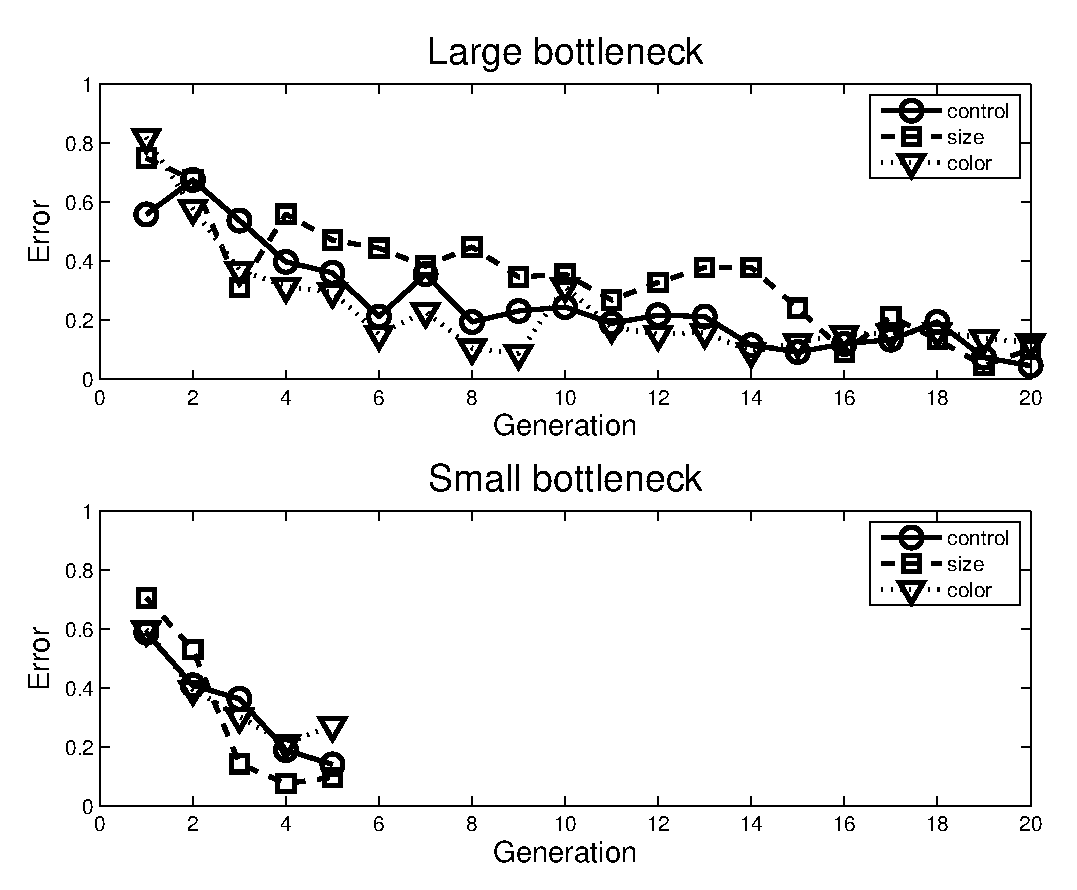
\includegraphics[scale=0.5]{convergence.eps}
\end{center}
\vspace{-5mm}
\caption{Transmission error by generation in each condition. As predicted, languages evolve to be increasingly learnable (decreasing transmission error in later generations),  and convergence is faster when the bottleneck is smaller. Note that the slightly lower convergence in the {\sc color} condition with the {\sc small} bottleneck is entirely carried by the final participant in one of the chains (Chain A).}
\label{fig:convergence}
\end{figure}

\vspace{5mm}
------------------------------ Insert Figure~\ref{fig:convergence} about here -------------------------------
\vspace{5mm}


 It is clear from Fig.~\ref{fig:convergence} that in all conditions, the chains ultimately converged to a low error rate. Convergence was slower in the {\sc large} bottleneck group, as predicted.

\begin{figure}
\begin{center}
\begin{tabular}{cc}
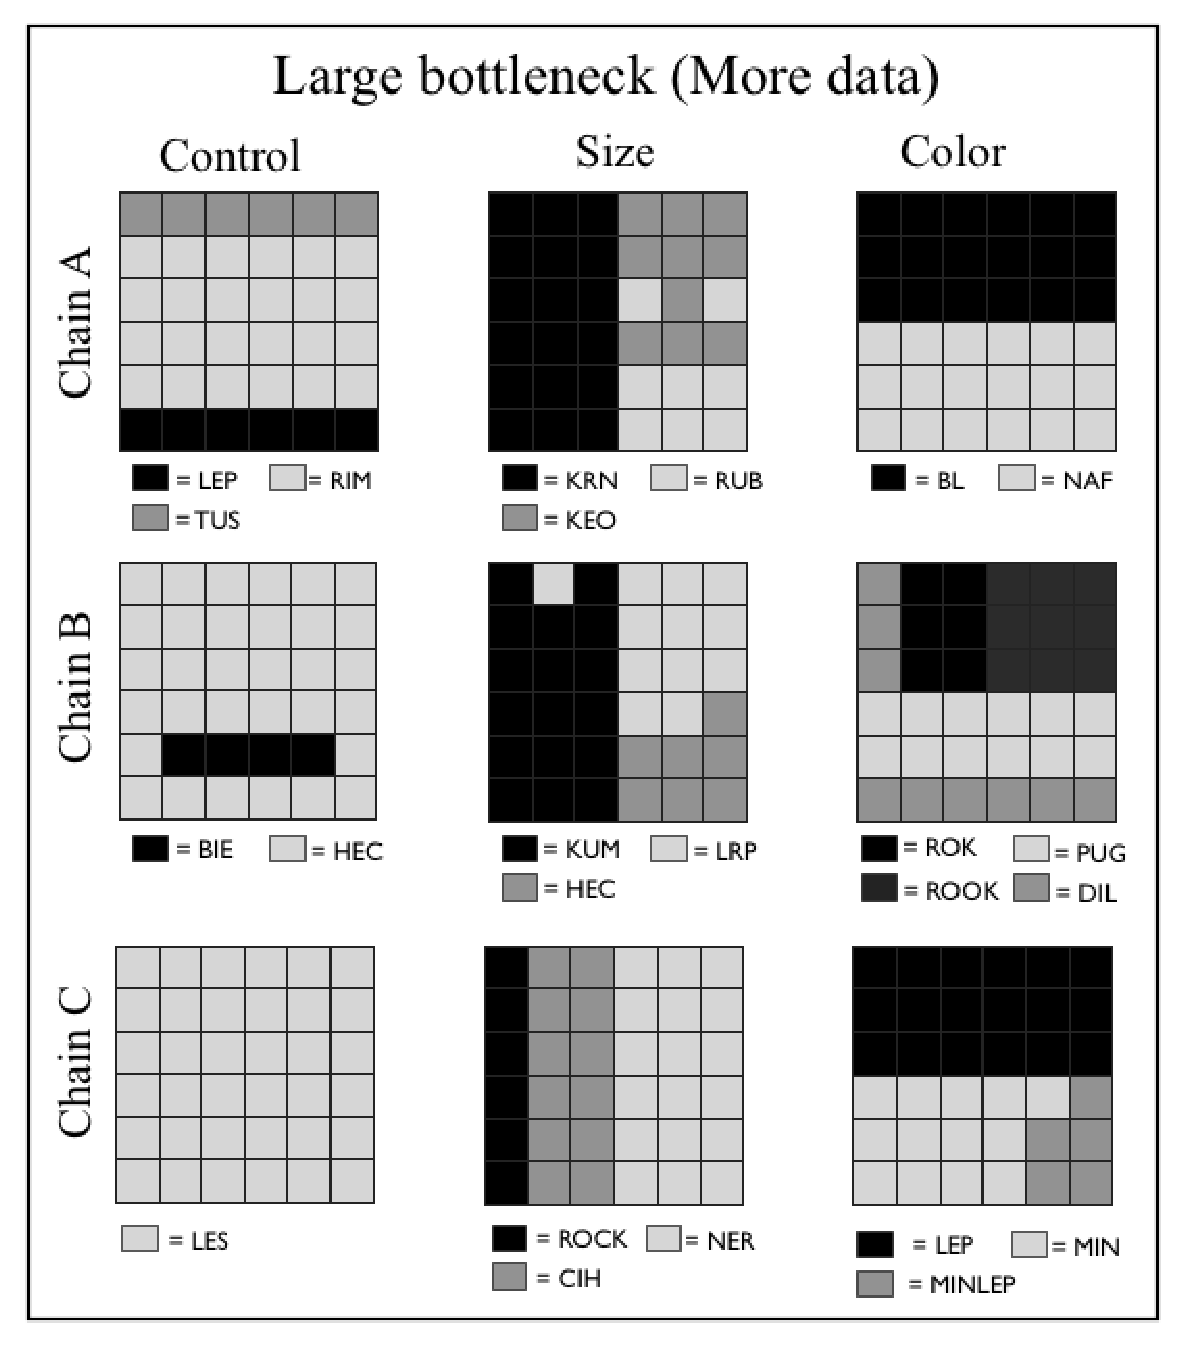
\includegraphics[scale=0.4]{largebottleneckall3.eps} &
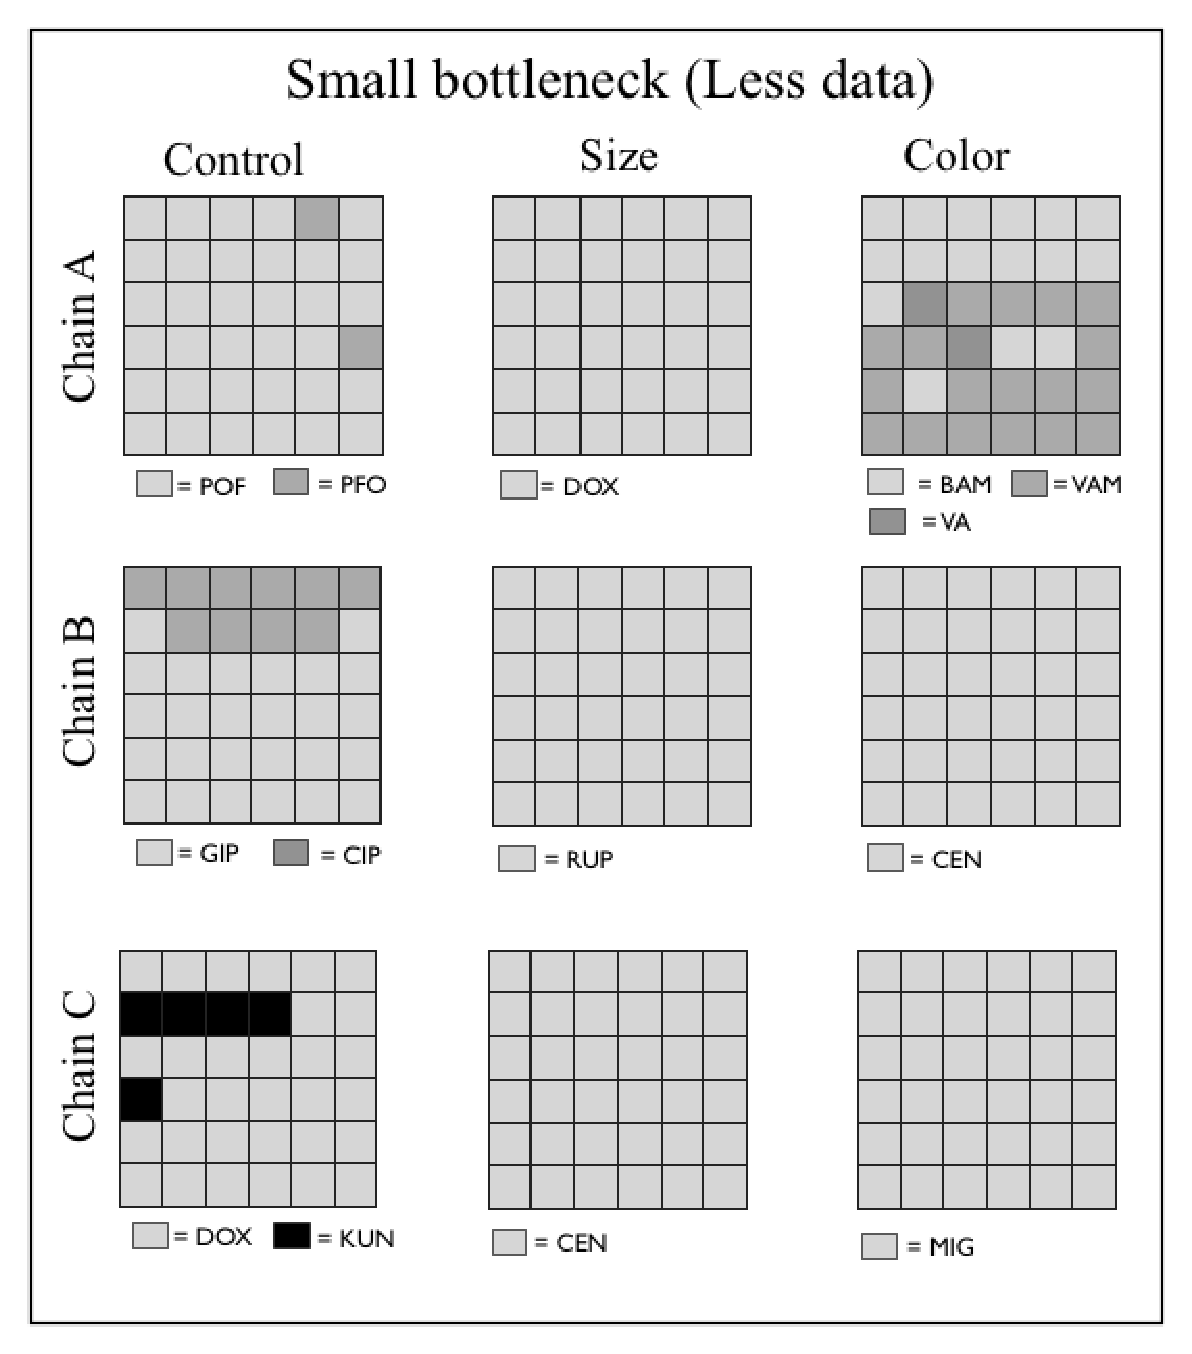
\includegraphics[scale=0.4]{smallbottleneck2.eps} \\
\end{tabular}
\end{center}
\vspace{-5mm}
\caption{Languages from the final participant in each of the chains in the {\sc large} and {\sc small} bottleneck groups. Each square is laid out as in Fig.\ref{fig:circles}, where the $y$ axis is size and the $x$ axis is color. Items labeled with the same word are depicted with the same shade; words that are very similar but not identical are depicted with similar shades. Specific words are detailed below each square. It is evident that in the {\sc large} bottleneck group, as predicted, the stimulus space has a considerable impact on the structure of the resulting language. All languages in the {\sc size} condition evolved words that categorized more according to size, all languages in the {\sc color} condition categorized more according to color, and all languages in the {\sc control} condition were not strongly driven by either dimension. Also as predicted, in the {\sc small} bottleneck group all languages evolved similarly; there was not enough data at each generation for the structure of the meaning space to affect how the languages evolved.}
\label{fig:individuals}
\end{figure}

\vspace{5mm}
------------------------------ Insert Figure~\ref{fig:individuals} about here -------------------------------
\vspace{5mm}


Our main prediction was that the structure of the world would affect the languages when the bottleneck was {\sc large} but not {\sc small}, since in the former case the data would exist in sufficiently high quantity that the stationary distribution would be closer to the expected posterior distribution, which includes the distribution of events in the world $Q(x)$. The results, shown in Fig.~\ref{fig:individuals}, are consistent with this prediction. In the {\sc large} bottleneck groups it is evident that there was a substantial effect of the structure of the meaning space on the structure of the resulting languages; all chains in the {\sc size} condition evolved words whose primary categorization divided the stimuli by size, and all chains in the {\sc color} condition evolved words which categorized according to color (although this effect was stronger for some chains than others).  By contrast, languages in the {\sc small} bottleneck groups tended to evolve towards having only one word, and there are no observable effects of world structure.

These differences can be quantified using the adjusted Rand Index or {\it adjR} \cite{hubertarabie85}. This measure captures the similarity between clusterings; an {\it adjR} of 1 indicates that the clusters are identical, while 0 is the score one would expect when comparing two random clusterings; scores below 0 indicate that the clusters match less than one would expect by chance.  Here, each of the resulting languages corresponds to one ``clustering'' of the stimuli; for instance, the language in Chain A of the {\sc color} condition in the {\sc large} bottleneck group corresponds to a clustering in which the 18 darkest stimuli are in one cluster and the 18 lightest stimuli are in another. We can compare each of the actual clusterings to the canonical color and size clusterings in Fig.~\ref{fig:exptstimuli}(b). The results are shown in Fig.~\ref{fig:adjR}. When the bottleneck is {\sc large}, the languages in the {\sc color} condition have a much higher {\it adjR} when compared to the canonical color clustering, and languages in the {\sc size} condition have a much higher {\it adjR} when compared to the canonical size clustering. However, in the {\sc small} bottleneck groups none of the languages are consistent with either canonical clustering.

\vspace{5mm}
------------------------------ Insert Figure~\ref{fig:adjR} about here -------------------------------
\vspace{5mm}

In order to determine if these results are significant, for each condition and bottleneck group we calculated a {\it structural precision score}, which captures the degree to which the evolved languages in each condition differentially match either the canonical color or canonical size clusterings. This score is given by the absolute value of the difference between the {\it adjR} value of that language for the canonical color clustering and its {\it adjR} value for the canonical size clustering.\footnote{The reason we calculate the statistics based on this score, rather than on something more intuitive like the {\it adjR} values themselves, is that the {\it adjR} values are not all independent of each other; e.g., if a language is highly consistent with the canonical size clustering, then it will not be consistent with the canonical color clustering. The {\it structural precision score}, by combining both values into one measure, ensures that all of the values entering into the statistical test are independent of each other.} If the {\it structural precision score} is close to zero, it indicates that the evolved language fits with both the canonical color and canonical size clusterings equally well -- in other words, that it has not evolved specifically to match either the size or color cluster. A higher {\it structural precision score} indicates that the language matches one of the two clusterings  better than the other -- in other words, that it has evolved to fit one ``world'' more than the other. If the structure of the world did have a significant role on the structure of the language, we would therefore expect that the {\it structural precision score} would be significantly higher in the {\sc color} and {\sc size} conditions (where the {\it adjR} values capturing the consistency of the language to the canonical size and canonical color should be markedly different from each other) than in the {\sc control} condition (where those {\it adjR} values should be similar). Moreover, we should expect to see this only in the {\sc large} bottleneck group, where the effect of world structure should be discernible.


As expected, the mean values of the {\it structural precision score} are larger in the {\sc size} and {\sc color} conditions than in the {\sc control} conditions when the bottleneck is large ({\sc size}: 0.685, {\sc color}: 0.670, {\sc control}: 0.055) but not when the bottleneck is small ({\sc size}: 0.0, {\sc color}: 0.117, {\sc control}: 0.109). A two-way ANOVA on bottleneck $\times$ condition reveals a significant main effect of bottleneck type ($F(1,12)=15.988, p=0.002$) and a significant interaction ($F(2,12)=5.333, p=0.022$). The nature of the interaction is evident in planned comparisons, which show that in the {\sc large} bottleneck group there is a significant effect of condition ($F(2,6)=6.155, p=0.035$) but in the {\sc small} bottleneck group there is not ($F(2,6)=0.528, p=0.615$). Together, these analyses indicate that, as predicted, the structure of the world has a significant effect on the structure of the language when the bottleneck is {\sc large} but not when it is {\sc small}.

% MAIN ANOVA
% > anova.all <- aov(diffval ~ adjRtype + condition + condition*adjRtype, data=data)
% > summary(anova.all)
%                    Df Sum Sq Mean Sq F value  Pr(>F)
% adjRtype            1 0.6991  0.6991  15.988 0.00177 **
% condition           2 0.3348  0.1674   3.829 0.05176 .
% adjRtype:condition  2 0.4664  0.2332   5.333 0.02202 *
% Residuals          12 0.5247  0.0437
% ---
% Signif. codes:  0 ?***? 0.001 ?**? 0.01 ?*? 0.05 ?.? 0.1 ? ? 1
%
% TESTING NORMALITY
% > residuals.all <- residuals(object=anova.all)
% > shapiro.test(x=residuals.all)
%
%	Shapiro-Wilk normality test
% data:  residuals.all
% W = 0.9557, p-value = 0.5208
%
%
% BREAK IT DOWN TO SMALL CONDITION
%
% > small <- subset(x=data,subset=data$adjRtype=="small")
% > anova.small <- aov(diffval ~ condition, data=small)
% > summary(anova.small)
%            Df  Sum Sq Mean Sq F value Pr(>F)
%condition    2 0.02583 0.01291   0.528  0.615
%Residuals    6 0.14676 0.02446
%
% BREAK IT DOWN TO LARGE CONDITION
% > large <- subset(x=data,subset=data$adjRtype=="large")
% > anova.large <- aov(diffval ~ condition, data=large)
% > summary(anova.large)
%            Df Sum Sq Mean Sq F value Pr(>F)
%condition    2 0.7753  0.3877   6.155 0.0352 *
% Residuals    6 0.3779  0.0630



\begin{figure}
\begin{center}
\includegraphics[scale=0.45]{adjrandvalues3.png}
\end{center}
\vspace{-5mm}
\caption{Average {\it adjR} values for the final languages in each condition, compared to the canonical clusterings according to size and color: an {\it adjR} of 0 indicates that they match no more than would be expected by chance, while an {\it adjR} of 1 indicates perfect alignment. In the {\sc large bottleneck} condition, the languages in the {\sc size} and {\sc color} conditions match their respective canonical clusterings far above chance; all other languages do not match either clustering. Error bars reflect standard error.}
\label{fig:adjR}
\end{figure}


\section{Discussion}

Our work indicates that if there is no {\em a priori} assumption that a learner's hypotheses about languages are independent of the external world they inhabit, and the external world {\it does} actually affect which events or meanings are spoken of, then the languages evolved by Bayesian learners through iterated learning will converge to a distribution that depends on the posterior probability over languages as well as the external structure of the meaning space. Here we consider some of the implications and limitations of our findings.

These results differ significantly from previous results by \citeA{griffithskalish05,griffithskalish07} that suggest that the stationary distribution of a chain of Bayesian iterated learners depends only on their prior.\footnote{Note that they are also distinct from (though related to) the results of \citeA{beppugriffiths09}, which reveal a different way that the stationary distribution of iterated learning can change when learners are provided with data generated by the external world. In that work, which is not focused on language, the hypotheses to be learned are hypotheses about the nature of the external distribution $x$ directly, rather than mappings between $x$ and $y$ (as occurs in language). Like us, \citeA{beppugriffiths09} find that the stationary distribution no longer converges to the prior, although the precise nature of the stationary distribution is not the same as we find here.}  This divergence arises because GK either assume that languages make no assumptions about the distribution of events in the world (2005) or that, if they do, the distribution of events spoken about is shaped entirely by the language and not at all by the external world (2007). Note that one cannot simply interpret GK's results in such a way that their sense of a prior itself includes these additional external environmental influences.
Interpreting the prior in such a way that it includes the structure of the world strips the GK result of much of its theoretical relevance: if one were to do this it would be impossible to distinguish between the effects of the cognitive biases of the learner and the effects of the environment in which the learner operates.

Since the difference between our results and GK's stems from different underlying premises about the relationship between the structure of the world and the nature of language, a natural question is which set of premises are correct. This is an open question, although we suggest that in at least some circumstances ours are plausible. First, the premise that the distribution of events $x$ that are talked about is shaped at least in part by the external structure of the world -- and not just by language -- seems eminently reasonable: we talk about cats not just because our language has the word ``cat'' but also because cats actually do exist, and we have direct experience of them. Second, the premise that languages make assumptions about the distribution of events in the world also appears sensible, at least sometimes. Language learners only start acquiring words after having observed many objects and events in the world, and it seems reasonable for them to expect word meanings to map onto these objects and events in a sensible way. The mapping between grammar and world structure is less obvious, but one might expect that learners' grammatical expectations are affected by their observations of the world -- for instance, expecting salient or frequent characteristics, like number or gender, to be marked grammatically, as has been suggested before \cite<e.g.,>{dubois87,bybee00,evans03}.  Further exploring in what circumstances this premise is correct is a subject for future research.

Our experimental results further support our theoretical predictions by showing that when people are exposed to different worlds with different distributions of events, the language that emerges reflects that event structure-- even when the people, as in most iterated learning experiments, do not realize that they are in the middle of ``evolving'' a language at all. It is important to note here that the experiments do {\it not} indicate, nor did we ever predict, that people's prior biases would play no role in shaping the structure of the language; in fact, it is quite likely that cognitive factors like memory are a major reason that languages in all conditions evolved to have fairly few words. Rather, the implication of the experiments is that world structure plays an {\it additional} role on top of the effect of whatever prior biases exist. This was evident in the fact that the difference between the evolved languages in {\sc size}, {\sc color}, and {\sc control} conditions can only be explained by the differences in the distribution of events $Q(x)$ in those conditions, since the participants were sampled from the same underlying population and thus presumably all shared similar prior biases.

There has been a great deal of experimental work supporting the finding that iterated learning experiments reveal human learners' inductive biases \cite{kirbyetal08,realigriffiths09,kalishetal07,griffithsetal08,smithwonnacott10}. How do we reconcile our results with this research? First, we do not deny that prior biases are a factor; our results simply suggest that in certain circumstances they are not the {\it only} factor. Second, our results do not invalidate the broad research program of using iterated learning experiments to illuminate people's inductive biases. Many experiments are constructed to either not have events be generated by the external world (i.e., have no $Q(x)$ distribution)
or to have all participants see the same distribution of events (i.e., they do not manipulate $Q(x)$ between conditions).
In such cases, one would still expect the stationary distribution to converge to the prior.
We do predict that significant changes in the distribution $Q(x)$ should result in different stationary distributions of the chains, although how large that effect may be in different kinds of experiments is an open empirical question.

Our findings may also resolve an apparent contradiction in the literature. While some theoretical results suggest that language evolution should converge to the prior, there is also theoretical work showing that the structure of the meaning space can affect the nature of the evolving language \cite{kirby01,brightonkirby01,smithetal03,mauritsetal10}. In addition, many empirical cross-linguistic results are consistent with the idea that aspects of world structure can affect linguistic structure.
Communicative complexity has been argued to increase with social complexity, both in humans and non-humans \cite{mccombsemple05,freebergetal12}, while phonological and morphological complexity may be negatively related to community size or isolation \cite{trudgill09,lupyandale10}. Others have suggested that environmental factors like frequency of use may also affect language structure \cite{bybee00,evans03}. While the link between some of these factors and the distribution $Q(x)$ that we are interpreting as world structure is not always exact, our work may help explain how these findings are possible in light of the GK results.

Further tests of our theoretical predictions will include additional cross-linguistic work as well as experimental, lab-based research -- for instance, varying the frequency of meanings and initializing chains with languages that do not match the space of meanings (e.g., initializing participants who see the meaning space from the {\sc color} condition with a language conforming to the canonical size pattern).
In addition, a great deal of theoretical work remains. Existing work investigates how GK's results are affected if the chain consists of more than one learner per generation \cite{smith09,burkettgriffiths10}, or if learners are capable of ``teaching'' subsequent learners in the chain \cite{beppugriffiths09}. How would our results be affected under these circumstances? Other work has built on the GK result to show that iterated learning with Bayesian learners is equivalent to the Wright-Fisher model of genetic drift \cite{realigriffiths09b}; does iterated learning correspond to a different evolutionary model when the stationary distribution it converges to is different?

There are many remaining open questions in addition to these, but our results indicate that the world may matter more than we previously thought. Perhaps language has the structure it does not just because of our brains, but because of the world as well.

\section{Acknowledgments}
We thank Natalie May, Tin Yim Chuk, Jia Ong, and Kym McCormick for their help recruiting participants and running the experiment, Simon Kirby and Mike Kalish for helpful discussions, and Tom Griffiths and Rick Dale for useful comments on a draft of the manuscript. AP and DJN were jointly supported by ARC fellowship DP0773794, AP individually by ARC fellowship DE120102378, and DJN individually by ARC fellowship FT110100431.

\section{Appendix A}

The derivation presented in the theoretical results is actually a special case of a more general derivation (we thank Tom Griffiths for a discussion of this).
This more general derivation diverges from the one in the main paper at step 4 below:

\footnotesize
\begin{eqnarray*}
\pi(h_{n+1})
&=& \sum_{h_n} P(h_{n+1} | h_n) \pi(h_n) \\
&=& \sum_{h_n} \sum_x \sum_y P(h_{n+1} | x, y) P(y | x, h_n) Q(x) \pi(h_n) \\
&=& \sum_{h_n} \sum_x \sum_y P(h_{n+1} | x, y) P(y | x, h_n) Q(x) \sum_{x^\prime} P(h_n | x^\prime) Q(x^\prime) \\
&=& \sum_{h_n} \sum_x \sum_y \frac{P(h_{n+1} | x) P(y | x, h_{n+1})}{\sum_{h^\prime} P(h^\prime | x) P(y|h^\prime,x)} P(y | x, h_n) Q(x) \sum_{x^\prime} P(h_n | x^\prime) Q(x^\prime) \\
&=& \sum_x P(h_{n+1}|x) Q(x) \left[ \sum_y P(y|h_{n+1},x) \frac{\sum_{h_n} (\sum_{x^\prime} P(h_n|x^\prime) Q(x^\prime)) P(y|h_n,x)}{\sum_{h^\prime} P(h^\prime|x)P(y|h^\prime,x)}\right] \\
\end{eqnarray*}
\normalsize

When the bracketed term is equal to 1, then $\pi(h_{n+1}) = \sum_x P(h_{n+1} | x) Q(x)$ (or, equivalently $\pi(h_n) = \sum_x P(h_n | x) Q(x)$). One circumstance when this occurs is, as in the main paper, when $P(h|x) \approx \sum_{x^\prime} P(h | x^\prime) Q(x^\prime)$:

\footnotesize
\begin{eqnarray*}
\pi(h_{n+1})
&=& \sum_x P(h_{n+1}|x) Q(x) \left[ \sum_y P(y|h_{n+1},x) \frac{\sum_{h_n} (\sum_{x^\prime} P(h_n|x^\prime) Q(x^\prime)) P(y|h_n,x)}{\sum_{h^\prime} P(h^\prime|x)P(y|h^\prime,x)}\right] \\
&=& \sum_x P(h_{n+1}|x) Q(x) \left[ \sum_y P(y|h_{n+1},x) \frac{\sum_{h_n} P(h_n|x) P(y|h_n,x)}{\sum_{h^\prime} P(h^\prime|x)P(y|h^\prime,x)}\right] \\
&=& \sum_x P(h_{n+1}|x) Q(x)
\end{eqnarray*}
\normalsize

There are presumably other circumstances under which the bracketed term is equal to 1, but they are much less straightforward and harder to offer an intuitive interpretation of. Because of this, and because the general point of the paper is simply that language evolution {\it can} be shaped by the structure of the world -- a point which is strengthened rather than weakened by this more general derivation -- our interpretation in the main paper focuses on the version presented there.

\renewcommand{\bibliographytypesize}{\footnotesize}
\bibliographystyle{apacite}

\setlength{\bibleftmargin}{.125in}
\setlength{\bibindent}{-\bibleftmargin}


%\bibliography{amy}

\begin{thebibliography}{}

\bibitem[\protect\citeauthoryear{%
Beppu%
\ \BBA{} Griffiths%
}{%
Beppu%
\ \BBA{} Griffiths%
}{%
{\protect\APACyear{2009}}%
}]{%
beppugriffiths09}%
\APACinsertmetastar{%
beppugriffiths09}%
Beppu, A.%
\BCBT{}\ \BBA{} Griffiths, T\BPBI L.%
%
\unskip\
\newblock
\APACrefYearMonthDay{2009}{}{}.
\newblock
\BBOQ{}\APACrefatitle{Iterated learning and the cultural rachet}{Iterated
  learning and the cultural rachet}.\BBCQ{}
\newblock
\BIn{} N.~Taatgen, H.~{van Rijn}, L.~Schomaker\BCBL{}\ \BBA{} J.~Nerbonne\
  (\BEDS), \APACrefbtitle{Proceedings of the 31st {A}nnual {C}onference of the
  {C}ognitive {S}cience {S}ociety}{Proceedings of the 31st {A}nnual
  {C}onference of the {C}ognitive {S}cience {S}ociety}\ (\BPG~2089-2094).
\newblock
\APACaddressPublisher{Austin, TX}{Cognitive Science Society}.
\PrintBackRefs{\CurrentBib}

\bibitem[\protect\citeauthoryear{%
Brighton%
\ \BBA{} Kirby%
}{%
Brighton%
\ \BBA{} Kirby%
}{%
{\protect\APACyear{2001}}%
}]{%
brightonkirby01}%
\APACinsertmetastar{%
brightonkirby01}%
Brighton, H.%
\BCBT{}\ \BBA{} Kirby, S.%
%
\unskip\
\newblock
\APACrefYearMonthDay{2001}{}{}.
\newblock
\APACrefbtitle{Meaning space structure determines the stability of culturally
  evolved compositional language}{Meaning space structure determines the
  stability of culturally evolved compositional language}\
  \APACbVolEdTR{}{\BTR{}}.
\newblock
\APACaddressInstitution{Language Evolution and Computation Research
  Unit}{University of Edinburgh}.
\PrintBackRefs{\CurrentBib}

\bibitem[\protect\citeauthoryear{%
Brighton%
, Smith%
\BCBL{}\ \BBA{} Kirby%
}{%
Brighton%
\ \protect\BOthers{.}}{%
{\protect\APACyear{2005}}%
}]{%
brightonetal05b}%
\APACinsertmetastar{%
brightonetal05b}%
Brighton, H.%
, Smith, K.%
\BCBL{}\ \BBA{} Kirby, S.%
%
\unskip\
\newblock
\APACrefYearMonthDay{2005}{}{}.
\newblock
\BBOQ{}\APACrefatitle{Language as an evolutionary system}{Language as an
  evolutionary system}.\BBCQ{}
\newblock
\APACjournalVolNumPages{Physics of Life Reviews}{2}{}{177-226}.
\PrintBackRefs{\CurrentBib}

\bibitem[\protect\citeauthoryear{%
Burkett%
\ \BBA{} Griffiths%
}{%
Burkett%
\ \BBA{} Griffiths%
}{%
{\protect\APACyear{2010}}%
}]{%
burkettgriffiths10}%
\APACinsertmetastar{%
burkettgriffiths10}%
Burkett, D.%
\BCBT{}\ \BBA{} Griffiths, T\BPBI L.%
%
\unskip\
\newblock
\APACrefYearMonthDay{2010}{}{}.
\newblock
\BBOQ{}\APACrefatitle{Iterated learning of multiple languages from multiple
  teachers}{Iterated learning of multiple languages from multiple
  teachers}.\BBCQ{}
\newblock
\BIn{} \APACrefbtitle{Proceedings of Evolang}{Proceedings of evolang}\
  (\BVOL~8).
\PrintBackRefs{\CurrentBib}

\bibitem[\protect\citeauthoryear{%
Bybee%
}{%
Bybee%
}{%
{\protect\APACyear{2000}}%
}]{%
bybee00}%
\APACinsertmetastar{%
bybee00}%
Bybee, J.%
%
\unskip\
\newblock
\APACrefYearMonthDay{2000}{}{}.
\newblock
\BBOQ{}\APACrefatitle{Lexicalization of sound change and alternating
  environments}{Lexicalization of sound change and alternating
  environments}.\BBCQ{}
\newblock
\BIn{} M.~Broe\ \BBA{} J.~Pierrehumbert\ (\BEDS), \APACrefbtitle{Papers in
  Laboratory Phonology V. Acquisition and the Lexicon}{Papers in laboratory
  phonology v. acquisition and the lexicon}\ (\BPGS\ 250--268).
\newblock
\APACaddressPublisher{Cambridge, UK}{Cambridge University Press}.
\PrintBackRefs{\CurrentBib}

\bibitem[\protect\citeauthoryear{%
Christiansen%
\ \BBA{} Chater%
}{%
Christiansen%
\ \BBA{} Chater%
}{%
{\protect\APACyear{2008}}%
}]{%
christiansenchater08}%
\APACinsertmetastar{%
christiansenchater08}%
Christiansen, M.%
\BCBT{}\ \BBA{} Chater, N.%
%
\unskip\
\newblock
\APACrefYearMonthDay{2008}{}{}.
\newblock
\BBOQ{}\APACrefatitle{Language as shaped by the brain}{Language as shaped by
  the brain}.\BBCQ{}
\newblock
\APACjournalVolNumPages{Behavioral and Brain Sciences}{31}{}{489-558}.
\PrintBackRefs{\CurrentBib}

\bibitem[\protect\citeauthoryear{%
{Du}~Bois%
}{%
{Du}~Bois%
}{%
{\protect\APACyear{1987}}%
}]{%
dubois87}%
\APACinsertmetastar{%
dubois87}%
{Du}~Bois, J.%
%
\unskip\
\newblock
\APACrefYearMonthDay{1987}{}{}.
\newblock
\BBOQ{}\APACrefatitle{The discourse basis of ergativity}{The discourse basis of
  ergativity}.\BBCQ{}
\newblock
\APACjournalVolNumPages{Language}{63}{}{805---855}.
\PrintBackRefs{\CurrentBib}

\bibitem[\protect\citeauthoryear{%
Evans%
}{%
Evans%
}{%
{\protect\APACyear{2003}}%
}]{%
evans03}%
\APACinsertmetastar{%
evans03}%
Evans, N.%
%
\unskip\
\newblock
\APACrefYearMonthDay{2003}{}{}.
\newblock
\BBOQ{}\APACrefatitle{Context, culture, and structuration in the languages of
  {A}ustralia}{Context, culture, and structuration in the languages of
  {A}ustralia}.\BBCQ{}
\newblock
\APACjournalVolNumPages{Annual Reviews in Anthropology}{32}{}{13--40}.
\PrintBackRefs{\CurrentBib}

\bibitem[\protect\citeauthoryear{%
Freeberg%
, Dunbar%
\BCBL{}\ \BBA{} Ord%
}{%
Freeberg%
\ \protect\BOthers{.}}{%
{\protect\APACyear{2012}}%
}]{%
freebergetal12}%
\APACinsertmetastar{%
freebergetal12}%
Freeberg, T.%
, Dunbar, R.%
\BCBL{}\ \BBA{} Ord, T.%
%
\unskip\
\newblock
\APACrefYearMonthDay{2012}{}{}.
\newblock
\BBOQ{}\APACrefatitle{Social complexity as a proximate and ultimate factor in
  communicative complexity}{Social complexity as a proximate and ultimate
  factor in communicative complexity}.\BBCQ{}
\newblock
\APACjournalVolNumPages{Philosophical Transactions of the Royal Society
  B}{367}{}{1785--1801}.
\PrintBackRefs{\CurrentBib}

\bibitem[\protect\citeauthoryear{%
Griffiths%
, Christian%
\BCBL{}\ \BBA{} Kalish%
}{%
Griffiths%
\ \protect\BOthers{.}}{%
{\protect\APACyear{2008}}%
}]{%
griffithsetal08}%
\APACinsertmetastar{%
griffithsetal08}%
Griffiths, T\BPBI L.%
, Christian, B.%
\BCBL{}\ \BBA{} Kalish, M.%
%
\unskip\
\newblock
\APACrefYearMonthDay{2008}{}{}.
\newblock
\BBOQ{}\APACrefatitle{Using category structures to test iterated learning as a
  method for identifying inductive biases}{Using category structures to test
  iterated learning as a method for identifying inductive biases}.\BBCQ{}
\newblock
\APACjournalVolNumPages{Cognitive Science}{31}{1}{68-107}.
\PrintBackRefs{\CurrentBib}

\bibitem[\protect\citeauthoryear{%
Griffiths%
\ \BBA{} Kalish%
}{%
Griffiths%
\ \BBA{} Kalish%
}{%
{\protect\APACyear{2005}}%
}]{%
griffithskalish05}%
\APACinsertmetastar{%
griffithskalish05}%
Griffiths, T\BPBI L.%
\BCBT{}\ \BBA{} Kalish, M.%
%
\unskip\
\newblock
\APACrefYearMonthDay{2005}{}{}.
\newblock
\BBOQ{}\APACrefatitle{A {B}ayesian view of language evolution by iterated
  learning}{A {B}ayesian view of language evolution by iterated
  learning}.\BBCQ{}
\newblock
\BIn{} B\BPBI G.~Bara, L\BPBI W.~Barsalou\BCBL{}\ \BBA{} M.~Bucciarelli\
  (\BEDS), \APACrefbtitle{Proceedings of the 27th {A}nnual {C}onference of the
  {C}ognitive {S}cience {S}ociety}{Proceedings of the 27th {A}nnual
  {C}onference of the {C}ognitive {S}cience {S}ociety}\ (\BPG~827-832).
\newblock
\APACaddressPublisher{Austin, TX}{Cognitive Science Society}.
\PrintBackRefs{\CurrentBib}

\bibitem[\protect\citeauthoryear{%
Griffiths%
\ \BBA{} Kalish%
}{%
Griffiths%
\ \BBA{} Kalish%
}{%
{\protect\APACyear{2007}}%
}]{%
griffithskalish07}%
\APACinsertmetastar{%
griffithskalish07}%
Griffiths, T\BPBI L.%
\BCBT{}\ \BBA{} Kalish, M.%
%
\unskip\
\newblock
\APACrefYearMonthDay{2007}{}{}.
\newblock
\BBOQ{}\APACrefatitle{Language Evolution by Iterated Learning With {B}ayesian
  Agents}{Language evolution by iterated learning with {B}ayesian
  agents}.\BBCQ{}
\newblock
\APACjournalVolNumPages{Cognitive Science}{31}{}{441-480}.
\PrintBackRefs{\CurrentBib}

\bibitem[\protect\citeauthoryear{%
Hauser%
, Chomsky%
\BCBL{}\ \BBA{} Fitch%
}{%
Hauser%
\ \protect\BOthers{.}}{%
{\protect\APACyear{2002}}%
}]{%
hauseretal02}%
\APACinsertmetastar{%
hauseretal02}%
Hauser, M.%
, Chomsky, N.%
\BCBL{}\ \BBA{} Fitch, W\BPBI T.%
%
\unskip\
\newblock
\APACrefYearMonthDay{2002}{}{}.
\newblock
\BBOQ{}\APACrefatitle{The faculty of language: What is it, who has it, and how
  did it evolve?}{The faculty of language: What is it, who has it, and how did
  it evolve?}\BBCQ{}
\newblock
\APACjournalVolNumPages{Science}{298}{5598}{1569--1579}.
\PrintBackRefs{\CurrentBib}

\bibitem[\protect\citeauthoryear{%
Hubert%
\ \BBA{} Arabie%
}{%
Hubert%
\ \BBA{} Arabie%
}{%
{\protect\APACyear{1985}}%
}]{%
hubertarabie85}%
\APACinsertmetastar{%
hubertarabie85}%
Hubert, L.%
\BCBT{}\ \BBA{} Arabie, P.%
%
\unskip\
\newblock
\APACrefYearMonthDay{1985}{}{}.
\newblock
\BBOQ{}\APACrefatitle{Comparing partitions}{Comparing partitions}.\BBCQ{}
\newblock
\APACjournalVolNumPages{Journal of Classification}{}{}{193--218}.
\PrintBackRefs{\CurrentBib}

\bibitem[\protect\citeauthoryear{%
Kalish%
, Griffiths%
\BCBL{}\ \BBA{} Lewandowsky%
}{%
Kalish%
\ \protect\BOthers{.}}{%
{\protect\APACyear{2007}}%
}]{%
kalishetal07}%
\APACinsertmetastar{%
kalishetal07}%
Kalish, M.%
, Griffiths, T\BPBI L.%
\BCBL{}\ \BBA{} Lewandowsky, S.%
%
\unskip\
\newblock
\APACrefYearMonthDay{2007}{}{}.
\newblock
\BBOQ{}\APACrefatitle{Iterated learning: Intergenerational knowledge
  transmission reveals inductive biases}{Iterated learning: Intergenerational
  knowledge transmission reveals inductive biases}.\BBCQ{}
\newblock
\APACjournalVolNumPages{Psychonomic Bulletin and Review}{14}{2}{288--294}.
\PrintBackRefs{\CurrentBib}

\bibitem[\protect\citeauthoryear{%
Kirby%
}{%
Kirby%
}{%
{\protect\APACyear{2001}}%
}]{%
kirby01}%
\APACinsertmetastar{%
kirby01}%
Kirby, S.%
%
\unskip\
\newblock
\APACrefYearMonthDay{2001}{}{}.
\newblock
\BBOQ{}\APACrefatitle{Spontaneous evolution of linguistic structure -- An
  iterated learning model of the emergence of regularity and
  irregularity}{Spontaneous evolution of linguistic structure -- an iterated
  learning model of the emergence of regularity and irregularity}.\BBCQ{}
\newblock
\APACjournalVolNumPages{IEEE Trans. on Evolutionary
  Computation}{5}{2}{102-110}.
\PrintBackRefs{\CurrentBib}

\bibitem[\protect\citeauthoryear{%
Kirby%
, Cornish%
\BCBL{}\ \BBA{} Smith%
}{%
Kirby%
\ \protect\BOthers{.}}{%
{\protect\APACyear{2008}}%
}]{%
kirbyetal08}%
\APACinsertmetastar{%
kirbyetal08}%
Kirby, S.%
, Cornish, H.%
\BCBL{}\ \BBA{} Smith, K.%
%
\unskip\
\newblock
\APACrefYearMonthDay{2008}{}{}.
\newblock
\BBOQ{}\APACrefatitle{Cumulative cultural evolution in the laboratory: An
  experimental approach to the origins of structure in human
  language}{Cumulative cultural evolution in the laboratory: An experimental
  approach to the origins of structure in human language}.\BBCQ{}
\newblock
\APACjournalVolNumPages{Proceedings of the National Academy of
  Sciences}{105}{31}{10681-10686}.
\PrintBackRefs{\CurrentBib}

\bibitem[\protect\citeauthoryear{%
Kirby%
\ \BBA{} Hurford%
}{%
Kirby%
\ \BBA{} Hurford%
}{%
{\protect\APACyear{2002}}%
}]{%
kirbyhurford02}%
\APACinsertmetastar{%
kirbyhurford02}%
Kirby, S.%
\BCBT{}\ \BBA{} Hurford, J.%
%
\unskip\
\newblock
\APACrefYearMonthDay{2002}{}{}.
\newblock
\BBOQ{}\APACrefatitle{The emergence of linguistic structure: An overview of the
  iterated learning model}{The emergence of linguistic structure: An overview
  of the iterated learning model}.\BBCQ{}
\newblock
\BIn{} A.~Cangelosi\ \BBA{} D.~Parisi\ (\BEDS), \APACrefbtitle{Simulating the
  evolution of language}{Simulating the evolution of language}\ (\BPGS\
  121--148).
\newblock
\APACaddressPublisher{London}{Springer Verlag}.
\PrintBackRefs{\CurrentBib}

\bibitem[\protect\citeauthoryear{%
Komarova%
\ \BBA{} Nowak%
}{%
Komarova%
\ \BBA{} Nowak%
}{%
{\protect\APACyear{2001}}%
}]{%
komarovanowak01}%
\APACinsertmetastar{%
komarovanowak01}%
Komarova, N.%
\BCBT{}\ \BBA{} Nowak, M.%
%
\unskip\
\newblock
\APACrefYearMonthDay{2001}{}{}.
\newblock
\BBOQ{}\APACrefatitle{Natural selection of the critical period for language
  acquisition}{Natural selection of the critical period for language
  acquisition}.\BBCQ{}
\newblock
\APACjournalVolNumPages{Proceedings of the Royal Society B}{268}{}{1189--1196}.
\PrintBackRefs{\CurrentBib}

\bibitem[\protect\citeauthoryear{%
Landau%
, Smith%
\BCBL{}\ \BBA{} Jones%
}{%
Landau%
\ \protect\BOthers{.}}{%
{\protect\APACyear{1988}}%
}]{%
landauetal88}%
\APACinsertmetastar{%
landauetal88}%
Landau, B.%
, Smith, L.%
\BCBL{}\ \BBA{} Jones, S.%
%
\unskip\
\newblock
\APACrefYearMonthDay{1988}{}{}.
\newblock
\BBOQ{}\APACrefatitle{The importance of shape in early lexical learning}{The
  importance of shape in early lexical learning}.\BBCQ{}
\newblock
\APACjournalVolNumPages{Cognitive Development}{3}{}{299--321}.
\PrintBackRefs{\CurrentBib}

\bibitem[\protect\citeauthoryear{%
Levenshtein%
}{%
Levenshtein%
}{%
{\protect\APACyear{1966}}%
}]{%
levenshtein66}%
\APACinsertmetastar{%
levenshtein66}%
Levenshtein, V.%
%
\unskip\
\newblock
\APACrefYearMonthDay{1966}{}{}.
\newblock
\BBOQ{}\APACrefatitle{Binary codes capable of correcting deletions, insertions,
  and reversals}{Binary codes capable of correcting deletions, insertions, and
  reversals}.\BBCQ{}
\newblock
\APACjournalVolNumPages{Soviet Physics Doklady}{6}{}{707-710}.
\PrintBackRefs{\CurrentBib}

\bibitem[\protect\citeauthoryear{%
Lupyan%
\ \BBA{} Dale%
}{%
Lupyan%
\ \BBA{} Dale%
}{%
{\protect\APACyear{2010}}%
}]{%
lupyandale10}%
\APACinsertmetastar{%
lupyandale10}%
Lupyan, G.%
\BCBT{}\ \BBA{} Dale, R.%
%
\unskip\
\newblock
\APACrefYearMonthDay{2010}{}{}.
\newblock
\BBOQ{}\APACrefatitle{Language structure is partly determined by social
  structure}{Language structure is partly determined by social
  structure}.\BBCQ{}
\newblock
\APACjournalVolNumPages{PLoS ONE}{5}{1}{e8559}.
\PrintBackRefs{\CurrentBib}

\bibitem[\protect\citeauthoryear{%
Maurits%
, Perfors%
\BCBL{}\ \BBA{} Navarro%
}{%
Maurits%
\ \protect\BOthers{.}}{%
{\protect\APACyear{2010}}%
}]{%
mauritsetal10}%
\APACinsertmetastar{%
mauritsetal10}%
Maurits, L.%
, Perfors, A.%
\BCBL{}\ \BBA{} Navarro, D\BPBI J.%
%
\unskip\
\newblock
\APACrefYearMonthDay{2010}{}{}.
\newblock
\BBOQ{}\APACrefatitle{Why are some word orders more common than others? {A}
  uniform information density account}{Why are some word orders more common
  than others? {A} uniform information density account}.\BBCQ{}
\newblock
\BIn{} \APACrefbtitle{{N}eural {I}nformation {P}rocessing {S}ystems}{{N}eural
  {I}nformation {P}rocessing {S}ystems}\ (\BVOL~23, \BPG~1585-1593).
\PrintBackRefs{\CurrentBib}

\bibitem[\protect\citeauthoryear{%
McComb%
\ \BBA{} Semple%
}{%
McComb%
\ \BBA{} Semple%
}{%
{\protect\APACyear{2005}}%
}]{%
mccombsemple05}%
\APACinsertmetastar{%
mccombsemple05}%
McComb, K.%
\BCBT{}\ \BBA{} Semple, S.%
%
\unskip\
\newblock
\APACrefYearMonthDay{2005}{}{}.
\newblock
\BBOQ{}\APACrefatitle{Coevolution of vocal communication and sociality in
  primates}{Coevolution of vocal communication and sociality in
  primates}.\BBCQ{}
\newblock
\APACjournalVolNumPages{Biological Letters}{1}{}{381---385}.
\PrintBackRefs{\CurrentBib}

\bibitem[\protect\citeauthoryear{%
Nowak%
, Komarova%
\BCBL{}\ \BBA{} Niyogi%
}{%
Nowak%
\ \protect\BOthers{.}}{%
{\protect\APACyear{2001}}%
}]{%
nowaketal01}%
\APACinsertmetastar{%
nowaketal01}%
Nowak, M.%
, Komarova, N.%
\BCBL{}\ \BBA{} Niyogi, P.%
%
\unskip\
\newblock
\APACrefYearMonthDay{2001}{}{}.
\newblock
\BBOQ{}\APACrefatitle{Evolution of universal grammar}{Evolution of universal
  grammar}.\BBCQ{}
\newblock
\APACjournalVolNumPages{Science}{291}{}{114-118}.
\PrintBackRefs{\CurrentBib}

\bibitem[\protect\citeauthoryear{%
Pinker%
\ \BBA{} Bloom%
}{%
Pinker%
\ \BBA{} Bloom%
}{%
{\protect\APACyear{1990}}%
}]{%
pinkerbloom90}%
\APACinsertmetastar{%
pinkerbloom90}%
Pinker, S.%
\BCBT{}\ \BBA{} Bloom, P.%
%
\unskip\
\newblock
\APACrefYearMonthDay{1990}{}{}.
\newblock
\BBOQ{}\APACrefatitle{Natural language and natural selection}{Natural language
  and natural selection}.\BBCQ{}
\newblock
\APACjournalVolNumPages{Behavioral and Brain Sciences}{13}{4}{707-784}.
\PrintBackRefs{\CurrentBib}

\bibitem[\protect\citeauthoryear{%
Reali%
\ \BBA{} Griffiths%
}{%
Reali%
\ \BBA{} Griffiths%
}{%
{\protect\APACyear{2009}}%
{\protect\APACexlab{{\protect\BCnt{1}}}}}]{%
realigriffiths09}%
\APACinsertmetastar{%
realigriffiths09}%
Reali, F.%
\BCBT{}\ \BBA{} Griffiths, T\BPBI L.%
%
\unskip\
\newblock
\APACrefYearMonthDay{2009{\protect\BCnt{1}}}{}{}.
\newblock
\BBOQ{}\APACrefatitle{The evolution of frequency distributions: Relating
  regularization to inductive biases through iterated learning}{The evolution
  of frequency distributions: Relating regularization to inductive biases
  through iterated learning}.\BBCQ{}
\newblock
\APACjournalVolNumPages{Cognition}{111}{}{317-328}.
\PrintBackRefs{\CurrentBib}

\bibitem[\protect\citeauthoryear{%
Reali%
\ \BBA{} Griffiths%
}{%
Reali%
\ \BBA{} Griffiths%
}{%
{\protect\APACyear{2009}}%
{\protect\APACexlab{{\protect\BCnt{2}}}}}]{%
realigriffiths09b}%
\APACinsertmetastar{%
realigriffiths09b}%
Reali, F.%
\BCBT{}\ \BBA{} Griffiths, T\BPBI L.%
%
\unskip\
\newblock
\APACrefYearMonthDay{2009{\protect\BCnt{2}}}{}{}.
\newblock
\BBOQ{}\APACrefatitle{Words as alleles: Connecting language evolution with
  {B}ayesian learners to models of genetic drift}{Words as alleles: Connecting
  language evolution with {B}ayesian learners to models of genetic
  drift}.\BBCQ{}
\newblock
\APACjournalVolNumPages{Proceedings of the Royal Society
  B}{277}{1680}{429-436}.
\PrintBackRefs{\CurrentBib}

\bibitem[\protect\citeauthoryear{%
K.~Smith%
}{%
K.~Smith%
}{%
{\protect\APACyear{2009}}%
}]{%
smith09}%
\APACinsertmetastar{%
smith09}%
Smith, K.%
%
\unskip\
\newblock
\APACrefYearMonthDay{2009}{}{}.
\newblock
\BBOQ{}\APACrefatitle{Iterated learning in populations of {B}ayesian
  agents}{Iterated learning in populations of {B}ayesian agents}.\BBCQ{}
\newblock
\BIn{} N.~Taatgen, H.~{van Rijn}, L.~Schomaker\BCBL{}\ \BBA{} J.~Nerbonne\
  (\BEDS), \APACrefbtitle{Proceedings of the 31st {A}nnual {C}onference of the
  {C}ognitive {S}cience {S}ociety}{Proceedings of the 31st {A}nnual
  {C}onference of the {C}ognitive {S}cience {S}ociety}\ (\BPGS\ 697--702).
\newblock
\APACaddressPublisher{Austin, TX}{Cognitive Science Society}.
\PrintBackRefs{\CurrentBib}

\bibitem[\protect\citeauthoryear{%
K.~Smith%
\ \BBA{} Wonnacott%
}{%
K.~Smith%
\ \BBA{} Wonnacott%
}{%
{\protect\APACyear{2010}}%
}]{%
smithwonnacott10}%
\APACinsertmetastar{%
smithwonnacott10}%
Smith, K.%
\BCBT{}\ \BBA{} Wonnacott, E.%
%
\unskip\
\newblock
\APACrefYearMonthDay{2010}{}{}.
\newblock
\BBOQ{}\APACrefatitle{Eliminating unpredictable variation through iterated
  learning}{Eliminating unpredictable variation through iterated
  learning}.\BBCQ{}
\newblock
\APACjournalVolNumPages{Cognition}{116}{}{444-449}.
\PrintBackRefs{\CurrentBib}

\bibitem[\protect\citeauthoryear{%
L.~Smith%
, Jones%
, Yoshida%
\BCBL{}\ \BBA{} Colunga%
}{%
L.~Smith%
\ \protect\BOthers{.}}{%
{\protect\APACyear{2003}}%
}]{%
smithetal03}%
\APACinsertmetastar{%
smithetal03}%
Smith, L.%
, Jones, S.%
, Yoshida, H.%
\BCBL{}\ \BBA{} Colunga, E.%
%
\unskip\
\newblock
\APACrefYearMonthDay{2003}{}{}.
\newblock
\BBOQ{}\APACrefatitle{Whose {DAM} account? {A}ttentional learning explains
  {B}ooth and {W}axman}{Whose {DAM} account? {A}ttentional learning explains
  {B}ooth and {W}axman}.\BBCQ{}
\newblock
\APACjournalVolNumPages{Cognition}{87}{}{209--213}.
\PrintBackRefs{\CurrentBib}

\bibitem[\protect\citeauthoryear{%
Trudgill%
}{%
Trudgill%
}{%
{\protect\APACyear{2009}}%
}]{%
trudgill09}%
\APACinsertmetastar{%
trudgill09}%
Trudgill, P.%
%
\unskip\
\newblock
\APACrefYearMonthDay{2009}{}{}.
\newblock
\BBOQ{}\APACrefatitle{Typology and Sociolinguistics: Linguistic Structure,
  Social Structure and Explanatory Comparative Dialectology}{Typology and
  sociolinguistics: Linguistic structure, social structure and explanatory
  comparative dialectology}.\BBCQ{}
\newblock
\APACjournalVolNumPages{Folia Linguistica}{31}{}{349--360}.
\PrintBackRefs{\CurrentBib}

\bibitem[\protect\citeauthoryear{%
Zuidema%
}{%
Zuidema%
}{%
{\protect\APACyear{2002}}%
}]{%
zuidema02}%
\APACinsertmetastar{%
zuidema02}%
Zuidema, W.%
%
\unskip\
\newblock
\APACrefYearMonthDay{2002}{}{}.
\newblock
\BBOQ{}\APACrefatitle{How the poverty of the stimulus solves the poverty of the
  stimulus}{How the poverty of the stimulus solves the poverty of the
  stimulus}.\BBCQ{}
\newblock
\BIn{} \APACrefbtitle{{N}eural {I}nformation {P}rocessing {S}ystems}{{N}eural
  {I}nformation {P}rocessing {S}ystems}\ (\BVOL~15).
\PrintBackRefs{\CurrentBib}

\end{thebibliography}



\end{document}




